\documentclass[12pt,a4paper,twoside]{ctexart}

%\usepackage{ctex}
%\usepackage{xeCJK}
\usepackage[utf8]{inputenc}


\usepackage{amsmath,amsthm,amssymb, slashed,upgreek,url,graphicx}

\usepackage[bookmarks=true,colorlinks,citecolor=black,linkcolor=black]{hyperref}
\usepackage{float}
\usepackage[svgnames]{xcolor}
\usepackage{subfig}
\usepackage{mathtools,nccmath}

\usepackage{fontspec}
\setCJKmainfont{FandolSong-Regular}[ BoldFont = FandolSong-Bold , ItalicFont = FandolKai-Regular ]



\numberwithin{figure}{section}

\numberwithin{equation}{section} 


\usepackage{listings}

\usepackage{fancyhdr}%页眉页脚宏包



\usepackage{geometry}%页面宏包
\geometry{a4paper,left=25mm,right=20mm,top=25mm,bottom=20mm}%设定页面
\pagestyle{fancy}%fancy 在geometry 后面
\fancyhf{}
\renewcommand{\headrulewidth}{0.15mm}%页眉线大小
\fancyhead[C]{作业报告}
\fancyfoot[RO,LE]{\thepage}
\setlength{\headheight}{15pt}
\linespread{1.5} %设定行距


\renewcommand{\contentsname}{目录} % default is {Contents}




\pagenumbering{Roman}

\title{{\bf\Huge 《2048》的艺术}\\ \normalsize 作业报告}
\date{2024 年 5 月 27 日}

\lstset{
    language=C++, % 设置语言
    basicstyle=\zihao{-5}\ttfamily, % 设置字体族
    breaklines=true, % 自动换行
    keywordstyle=\bfseries\color{magenta}, % 设置关键字为粗体,颜色
    morekeywords={COORD,HANDLE,DWORD,CONSOLE_CURSOR_INFO,string}, % 设置更多的关键字,用逗号分隔
    emph={std,cout,endl,rows,cols,GetConsoleScreenBufferInfo,SetConsoleMode,GetConsoleMode,SetConsoleCursorInfo,SetConsoleTextAttribute,SetConsoleCursorPosition,GetStdHandle,system}, % 指定强调词,如果有多个,用逗号隔开
    emphstyle=\bfseries\color{NavyBlue}, % 强调词样式设置
    commentstyle=\color{Green!90!black}, % 设置注释样式,斜体,浅灰色
    stringstyle=\bfseries\color{black!50!white}, % 设置字符串样式
    columns=fixed,  % 如果不加这一句,字间距就不固定,很丑,必须加
    basewidth=0.5em,
    numbers=left, % 显示行号在左边
    numberstyle=\zihao{-5}\ttfamily, % 缩小行号
    frame=lrtb, % 边框
}



\begin{document}
\maketitle
\setcounter{page}{0}
\thispagestyle{empty}

\newpage

\tableofcontents%目录


\newpage
\pagenumbering{arabic}

\section{概览}
\subsection{功能描述}


先呈现的是菜单界面,可供玩家选择经典模式、游戏规则或退出游戏.游戏使用方向键(↑←↓→)或 WASD 键操作,在游戏过程中可随时按 ESC 键退至菜单.游戏规则是,每选择一个方向移动,移动时数字向该方向靠拢;相同数字可合并,之后空格处会生成随机数字2/4;若得数字2048,则游戏胜利(其实部分官方版本无此提示);若棋盘被填满,无法进行移动,则游戏结束(不一定失败).

\begin{figure}[ht]
    \centering
    
\includegraphics[width=.45\textwidth]{menu.png}
    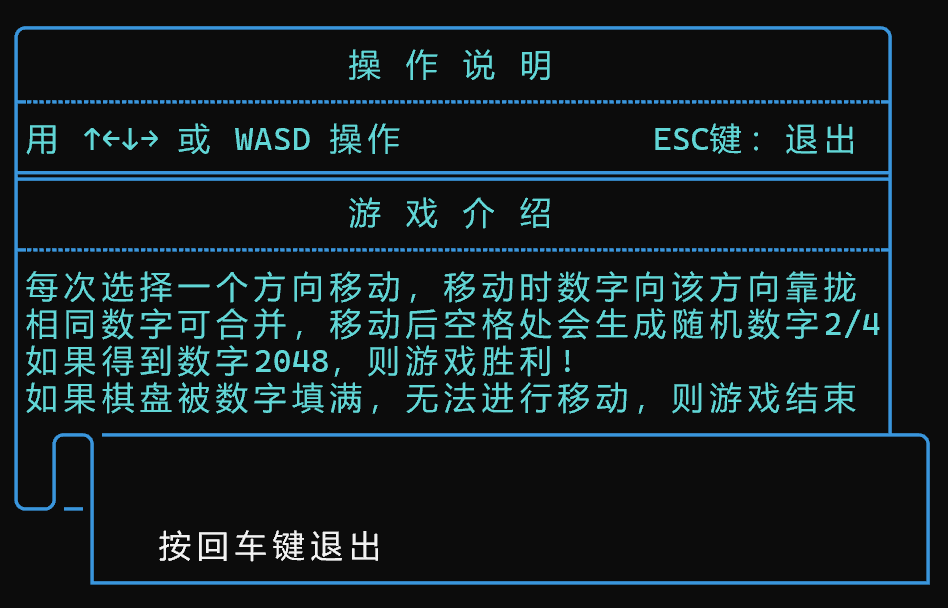
\includegraphics[width=.45\textwidth]{displayHelp.png}\\
    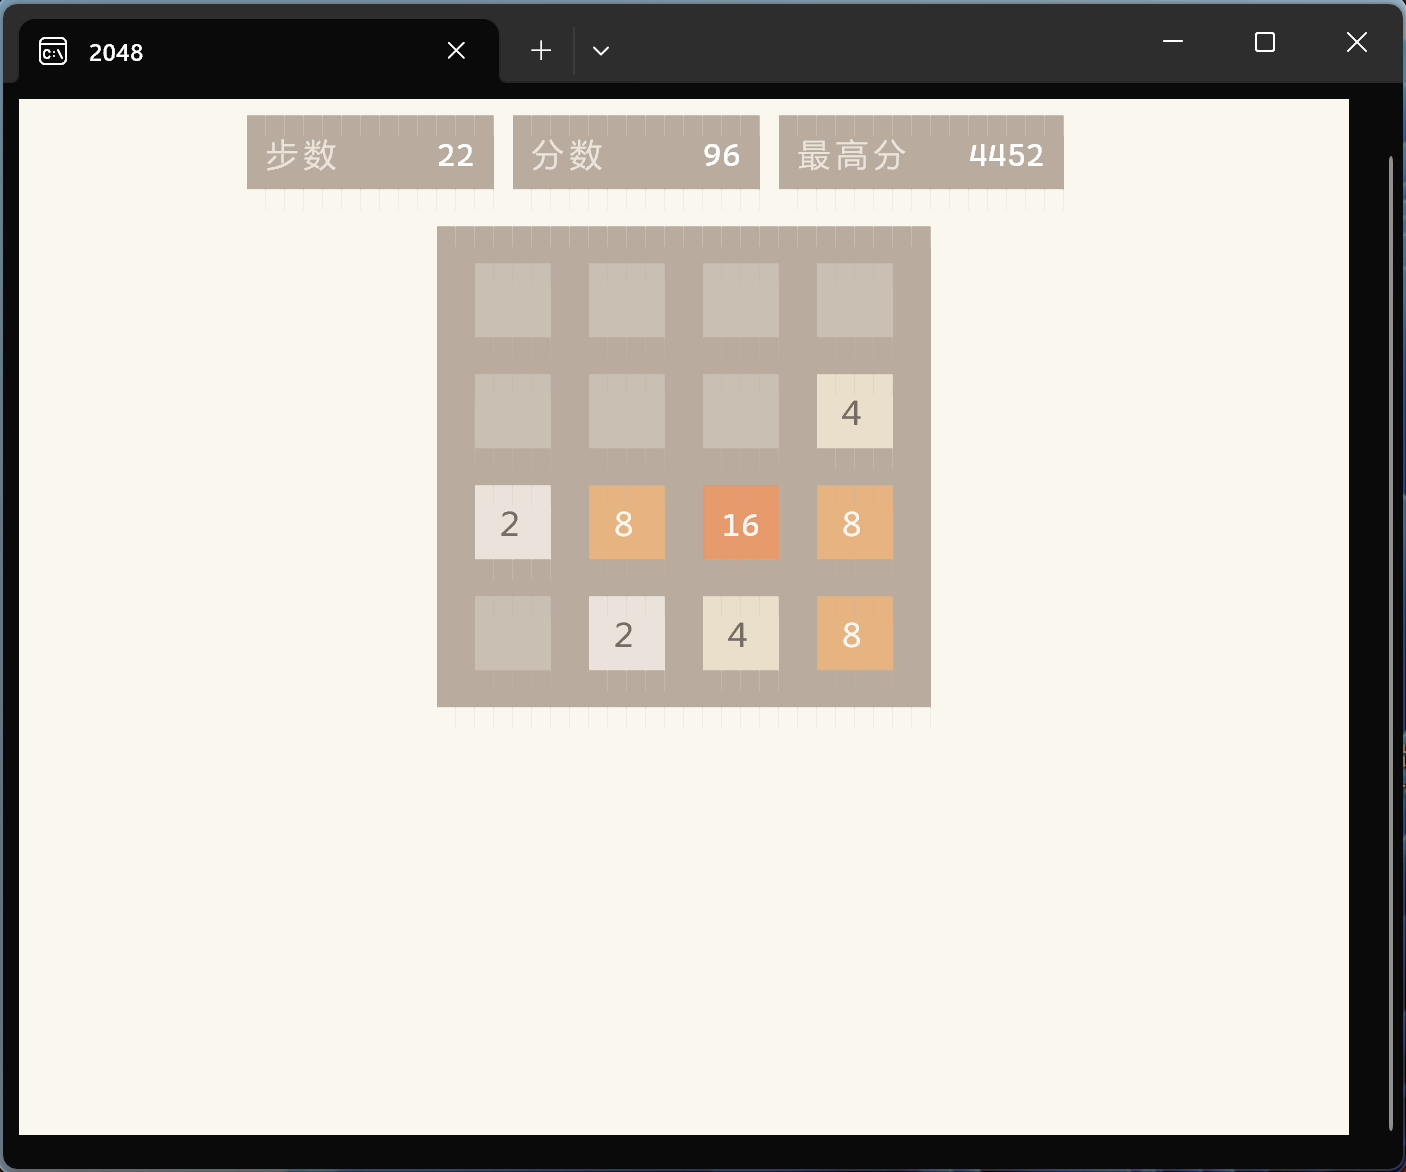
\includegraphics[width=.5\textwidth]{displayInterface.png}
    \caption{菜单、帮助、游戏画面}
\end{figure}

游戏提供三类计数器:步数、分数以及最高分.其中步数即产生方块移动的有效按键数,分数则只当合并时在原基础上增加该合并的数字,而最高分会存入一个 \verb|txt| 文件中(第一次游玩时自动生成).

此外,玩家操作时,游戏界面还将呈现出\textit{滑动}、\textit{合成}动画.

\begin{figure}[p]
    \centering
    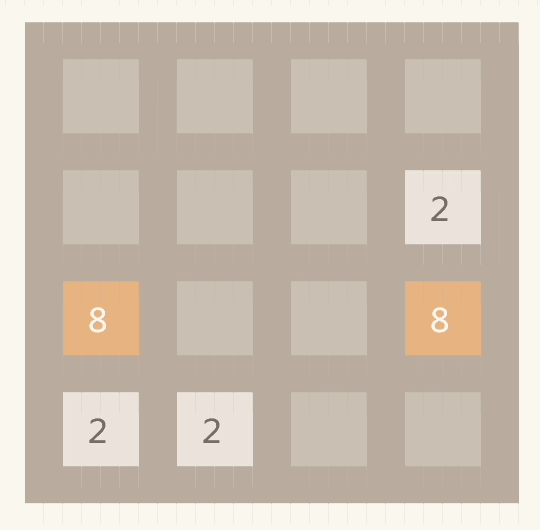
\includegraphics[width=.3\textwidth]{01.png}
    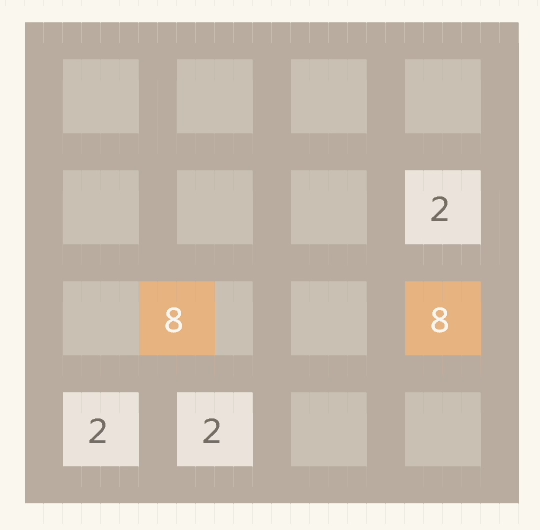
\includegraphics[width=.3\textwidth]{02.png}
    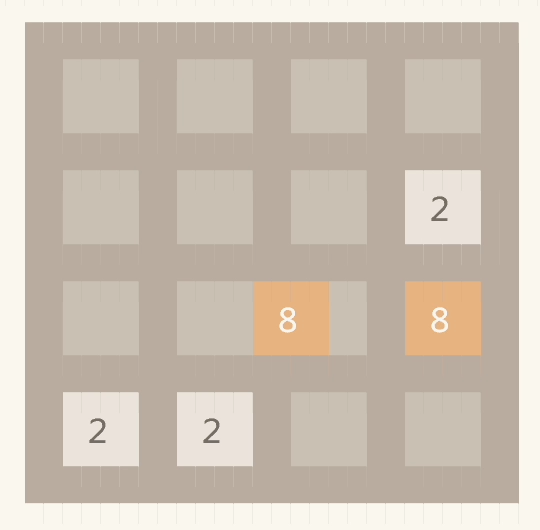
\includegraphics[width=.3\textwidth]{03.png}\\
    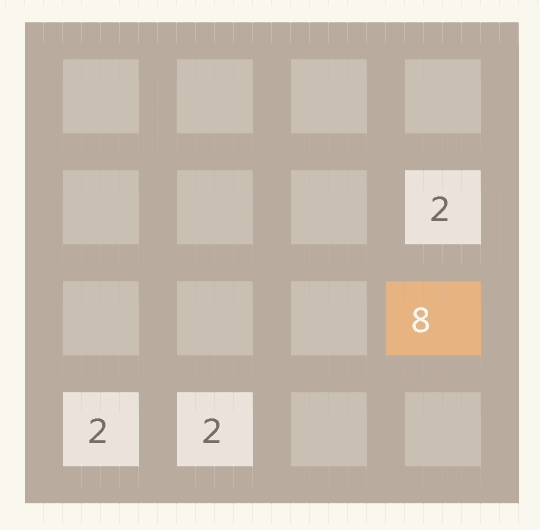
\includegraphics[width=.3\textwidth]{04.png}
    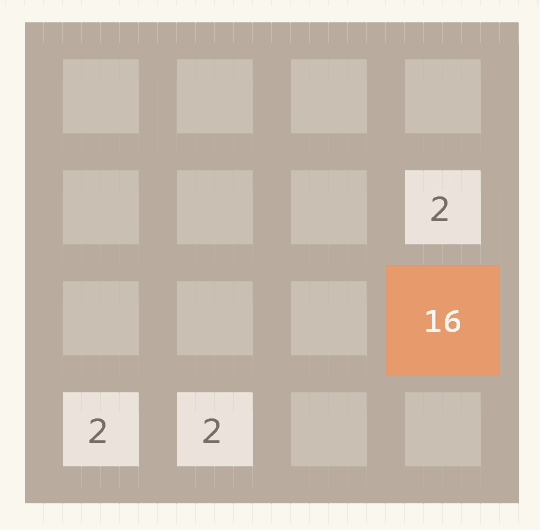
\includegraphics[width=.3\textwidth]{05.png}
    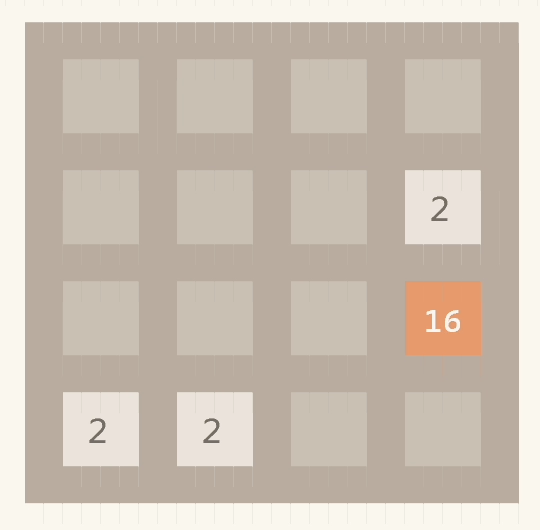
\includegraphics[width=.3\textwidth]{06.png}
    \caption{滑动及倍增特效.实际处理是逐字符滑动,帧数更高}
\end{figure}

\begin{figure}[p]
    \centering
    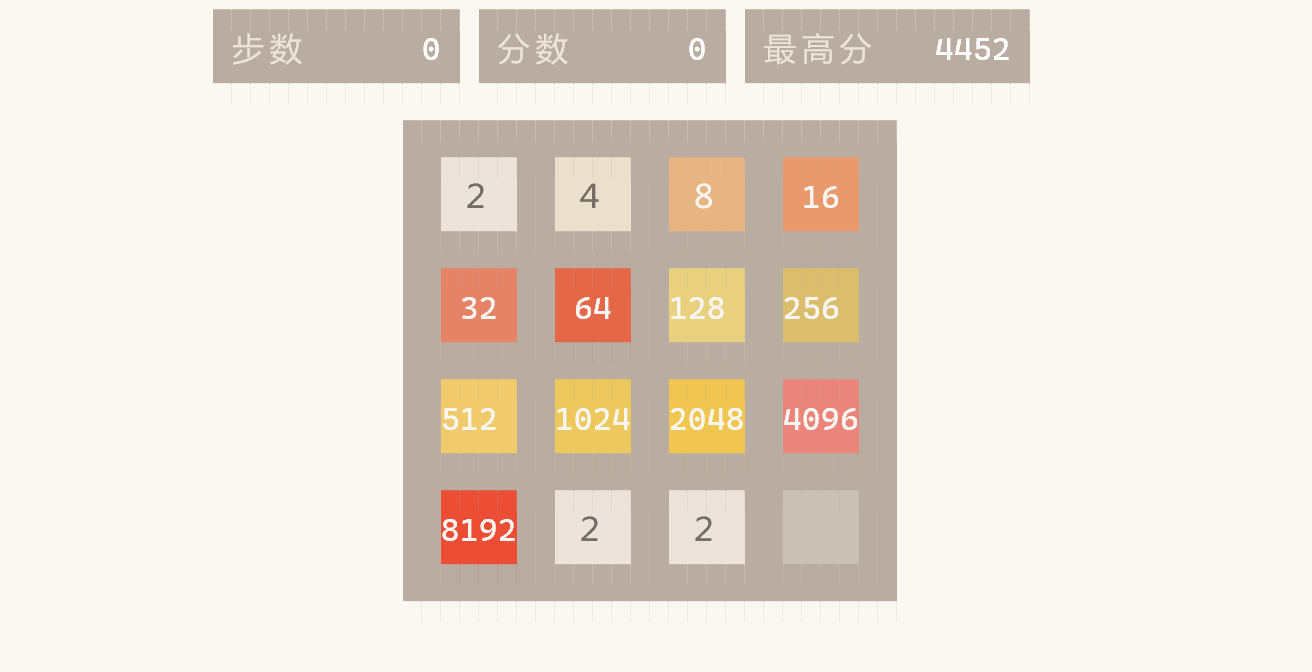
\includegraphics[width=.6\textwidth]{every.png}
    \caption{可支持的方块样式}
\end{figure}

\begin{figure}[p]
    \centering
    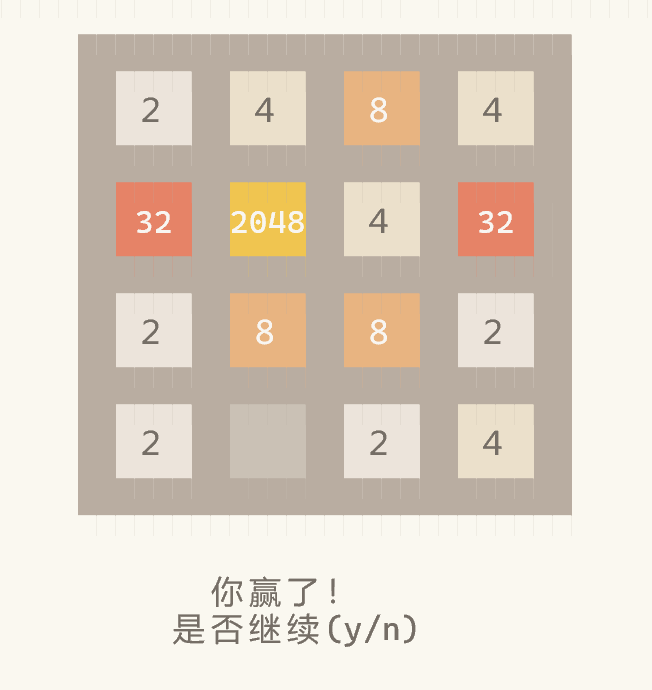
\includegraphics[width=.3\textwidth]{win.png}
    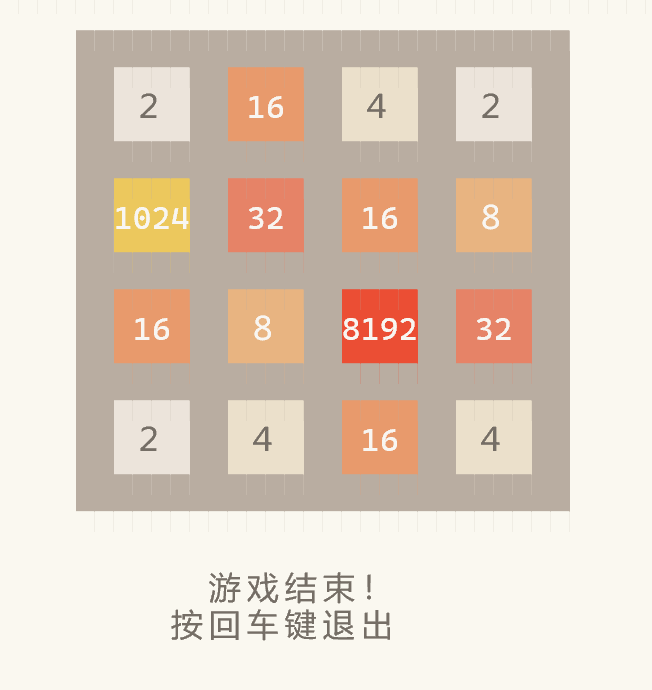
\includegraphics[width=.3\textwidth]{over.png}
    \caption{胜利和结束画面}
\end{figure}




\subsection{设计思路}
从菜单到游戏规则、退出机制的逻辑都很好处理.参考模版已给出了若干模块:回车键 \verb|wait_for_enter()|、菜单显示 \verb|print_menu()|、帮助显示 \verb|print_help()|、游戏界面显示 \verb|print_interface()|.

重头戏在游戏主循环.先定义基本变量(多数为 \verb|int|),如棋盘 \verb|board[4][4]|、分数 \verb|score|、步数 \verb|step|、最高分 \verb|high_score|、输赢状态 \verb|bool game_won|、可移动状态 \verb|bool can_move| 等.用 \verb|char choice| 记录用户按键 \verb|_getch()|.

游戏循环 \verb|play_game()| 大致需要如下模块:
\begin{itemize}
    \item 先用 \verb|background()| 涂满背景颜色,将 \verb|print_interface()| 强调为打印初始的空界面的作用
    \item 用 \verb|read_high_score()| 读取文件中的最高分.读取和写入文件都需要库 \verb|<fstream>|
    \item 刷新数据 \verb|update_board(board,score,step,high_score)|,其中步数、分数、最高分等数据可用 \verb|setw()| 固定位 6 位右对齐.
    \item 随机生成方块 \verb|add_random_tile(board)| 并播放动画.为了达到更好的随机效果,考虑用 \verb|<random>| 中的 \verb|gen()|.
    \item 此后用户进行操作,故要设置移动算法 \verb|move_tiles(board, choice, score)| 并播放动画.操作一次,再利用 \verb|update_board| 更新数据并用 \verb|add_random_tile| 生成方块,并检查最高分
    \item 先判断是否胜利(出现 2048),再判断是否可移动(不能移动则游戏结束)
    \item 无论是用户自主退出还是游戏结束,最后都要用 \verb|write_high_score(high_score)| 写入最高分
\end{itemize}

其次是关于绘制游戏界面、动画的细节.这需要一些额外的模块:
\begin{itemize}
    \item 首先是一些利用 Windows API 对控制台标准输出设备句柄的设置(除非编译器标准头文件里有这些函数),如基于 \verb|SetConsoleCursorPosition| 的指定坐标输出函数 \verb|gotoxy(x, y)|;基于 \verb|SetConsoleTextAttribute| 的指定颜色输出函数 \verb|color(c)|;基于 \verb|SetConsoleCursorInfo| 的隐藏光标函数 \verb|HideCursor()|,在程序开始时就使用
    \item 由于可能涉及更多在 \verb|color| 允许范围外的颜色(RGB 已足够),考虑使用 \textbf{ANSI 转义序列},即在程序开始时就设置好 \verb|ConsoleMode|,可整合为函数 \verb|enableAnsiSupport()|.这需要编译的系统为 Windows 10 的高版本、Windows 11
    \item 显示方块的函数为 \verb|display_tile(int x, int y, int num, int back)|,其中 \verb|back| 是考虑为方块设置背景的可能性
    \item 移动动画为 \verb|move_with_animation(x, y, char direction, num)|,合并\&倍增动画为 \verb|double_with_animation(x, y, direction, num)|.其中为了更精确的延迟时间,需要定义高精度延迟函数 \verb|high_precision_sleep(float time)|
\end{itemize}



\newpage
\section{问题及解决方法}
\subsection{控制台 API}
花了一些时间学习如何指定坐标输出、制定颜色输出,以及 ANSI 转义序列的操作机制,比如输出字符串 \verb|"\x1b[38;2;"| 代表前景(\verb|48| 代表背景),其后紧更 RGB 值,如 \verb|"255;234;0"|,最后用 \verb|"m"| 结尾,就代表一个 ANSI 指令,之后可以跟上你想输出的字符内容.如方块 2 的四字节显示的字符串为 \verb|\x1b[38;2;117;110;102;48;2;236;228;219m 2 |,其中“\verb|2|”是全角版本的 2.

\subsection{菜单选择}
直接按 a,b,c 的方式不太像是一个游戏该有的操作.一个更接近任天堂红白机(笑)的操作方式是用上下键选择不同选项.因此花了一些时间学习上下键选择、空格或回车确定的程序逻辑,其中用 \verb|enum| 类型记录了选项,最后用一个大于符号“\verb|>|”充当红色的小三角以指向当前选项.
\subsection{游戏帮助}
花了点时间绘制了类似于“一张信件”的界面,上面“写有”游戏帮助,如操作和规则.
\subsection{游戏界面}
重头戏……首先 2048 背景颜色在 \verb|color()| 范围外,因此只能用 ANSI 转义序列,而后者又不支持直接更换背景颜色,因此必须要先判断控制台窗口大小,再瞬间涂满.这些程序写在了 \verb|background()| 中.

2048 的操作算法、判断机制(即游戏主逻辑)对我倒无大碍,真正磨人的是显示部分.首先,为了得到不同方块,要用一个数组 \verb|tile_colors[]| 存储每个方块背景的 RGB 值.而这些值我必须要在 2048 的源码寻找,或直接用取色器在游戏界面(包括同人版本)中提取,十分繁琐.

滑动动画部分,我并不满足于逐个格子的跳动,我更想实现更为丝滑的“像素级”移动,即逐个字符.然而,由于我的棋盘使用了一些复杂的半角型\textbf{方框绘制字符},如图,好看是好看,但所谓“前端一笑、后端心凉”,在编写显示方块、移动动画、倍增动画三类模块时,我经历了痛不欲生的判断和调试,甚至为此画了三页草稿纸.

解决方法是什么?睡好吃好心情好,慢慢调慢慢捋清,自然就可以肝出来了.


\begin{figure}[ht]
    \centering
    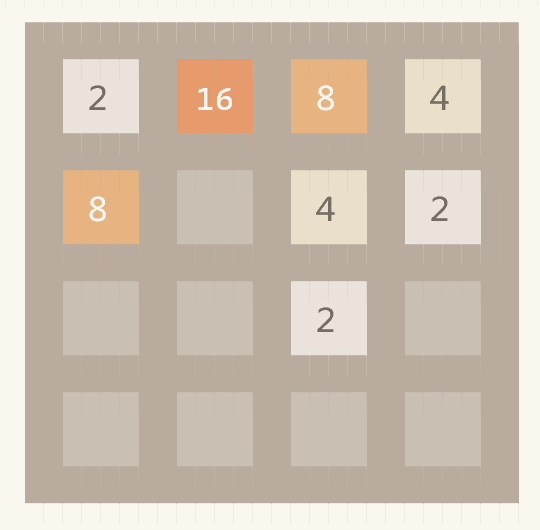
\includegraphics[width=.3\textwidth]{11.png}
    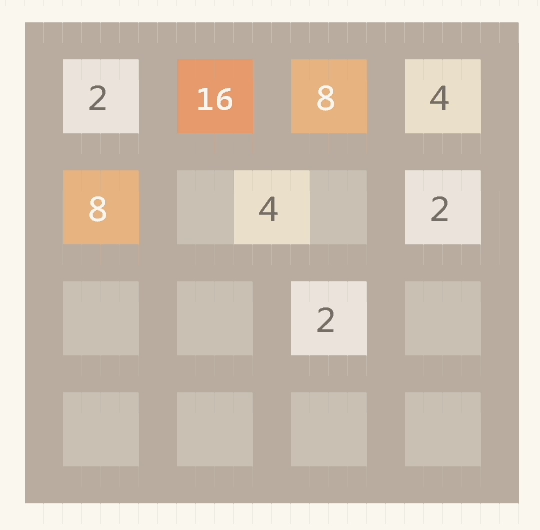
\includegraphics[width=.3\textwidth]{12.png}
    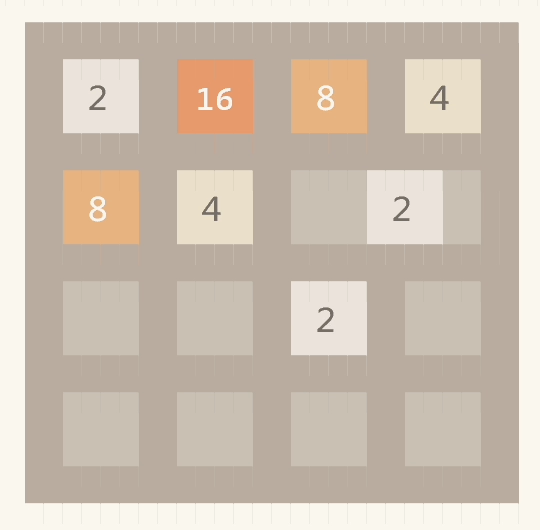
\includegraphics[width=.3\textwidth]{13.png}\\
    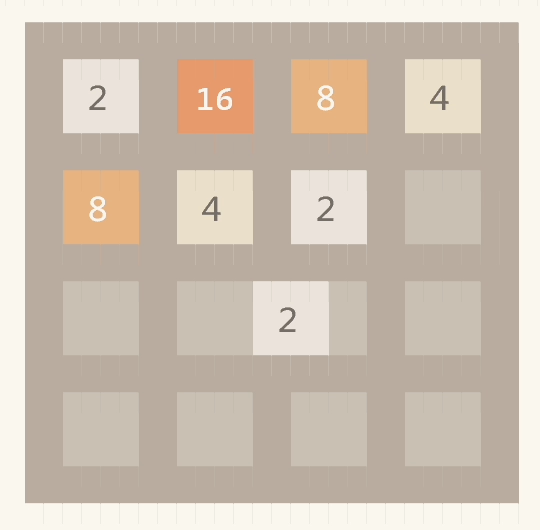
\includegraphics[width=.3\textwidth]{14.png}
    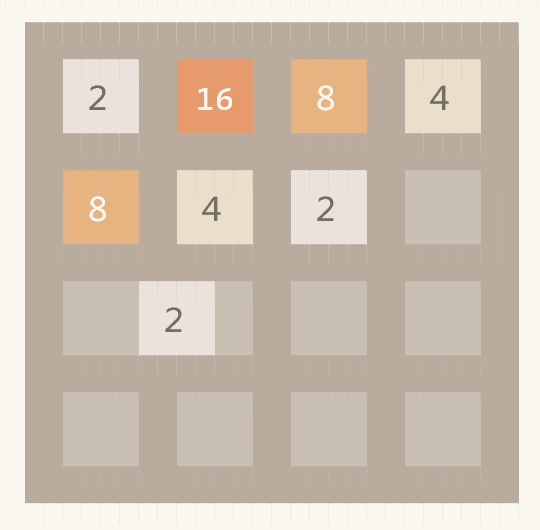
\includegraphics[width=.3\textwidth]{15.png}
    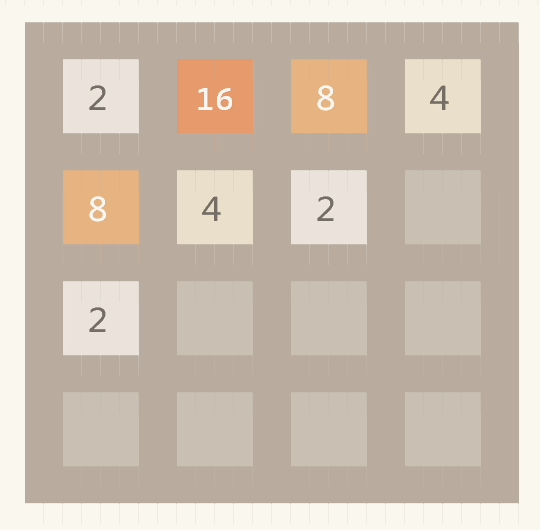
\includegraphics[width=.3\textwidth]{16.png}
    \caption{可见缺陷是需要每个方块依次地移动}
\end{figure}


具体来说,显示方块比较简单,只要别把 16 个方格的中心位置搞错即可;倍增动画也还好,我只要给方块加上一圈像素再恢复,就可模仿出方块突然放大并收缩的效果.由于我目前只考虑逐个方块的移动,因此我需要计算一个方块移动一格时,如何将其末尾的像素擦除并换上相应的背景像素.这就是重头戏中的重头戏.

一个更好的方式当然是考虑所有方块一齐地同时到达各自终点.这涉及改动大量的逻辑,并且为了方便最好要定义全局数组(我也不想用指针和在各自模块里重复定义).大致来说,需要预先设置一个二维数组用来存储当前棋盘状态的像素,每次计算下一步状态所需显示的像素,计算好再刷新整个棋盘,而不再拘泥于局部像素的刷新,这样也能达到多个方块的同步移动.不过这近似于用控制台重新写一个 \verb|graphics.h| 了(甚至可以让字体缩小,长宽一致,真正达到“像素级”绘图),工作量太大,时间紧迫,以后再说.

\newpage
\section{心得体会}
\subsection{算法设计及编码过程}
说实话,游戏主要的算法和编码并没有困扰我太多,何况现在还有 AI 加持,其实大量减轻了这类重复工作.然而,目前 AI 对前端的美化还很薄弱,因此关于前端的繁琐工作还是得靠我自己来……

\subsection{随机函数}
简单的伪随机数通常使用当前时间作为种子.然而如果需要短时间内给出两个随机数,这种伪随机往往将给出相同数字.一个更好的随机是利用更多的种子,如 \verb|gen()| 就是用随机设备作为种子.接近于“真随机”的过程需要设备芯片的物理底层设置,涉及固体物理和半导体物理.没错,芯片有专门的部分用于生成足够真实的随机数.按还原论主义来说,顶级芯片所采用的随机机制是默认了微观物理过程的一些信息丢失,如果理论上能得到我们想要的实验信息,其实仍可预测出结果.当然,目前 Newton 决定性原理和量子理论还未发展完善,我们并不清楚\textit{真正的}随机是否存在.只要这个随机对用户来说足够不可预测即可.

\subsection{游戏框架}
几乎所有游戏都要涉及一个大循环,用户在单个循环中走入不同的 \verb|if| 语句内的模块之中.

其实一款游戏最重要的还是美学、可玩性和文化等这些非编程的东西,也即用代码堆积起来的艺术.AI 想必还是能解放人在编程上的禁锢,而专心于创作之中,换言之,解放人在游戏底层的编程(乃至一些图形学算法),而专注于主题、灵感等.

\subsection{游戏攻略}
我并不是专家,但据传言,将当前的最大方块(如 512)放置于角落,并尽可能保证移动过程中不动它,且其余方块的大小朝一定蛇形或螺旋形排列,就容易按此路径一直合成,最终达到 2048 乃至 4096.

\subsection{所思所感及吐槽}
在前端开心设计,在后端悲愤骂娘.这些滑动、回弹、非线性动画好看是真好看,而写起来繁琐也是真繁琐.不知道 Apple 公司到底怎么活的,那么多 Gauss 模糊、毛玻璃、阴影、平面风格效果……

\newpage
\section{部分源代码}
只截取自己程序中核心或有亮点的代码.由于部分模块涉及到特殊字符,不便于直接编辑在文档里,故这些模块采取截图形式.
\subsection{控制台 API}
\begin{lstlisting}[
    caption     =   {在指定坐标输出字符},
]
void gotoxy(int x, int y) {
    COORD pos;
    pos.X = x;
    pos.Y = y;
    SetConsoleCursorPosition(GetStdHandle(STD_OUTPUT_HANDLE), pos);
}
\end{lstlisting}

\begin{lstlisting}[
    caption     =   {隐藏光标},
]
void HideCursor() {
    CONSOLE_CURSOR_INFO Cursor;
    Cursor.bVisible = FALSE;
    Cursor.dwSize = sizeof(Cursor); //如果没赋值的话,光标隐藏无效
    SetConsoleCursorInfo(GetStdHandle(STD_OUTPUT_HANDLE), &Cursor);
}
\end{lstlisting}

\begin{lstlisting}[
    caption     =   {设置字符串或单个字符的颜色及背景},
]
void color(int c) {
    SetConsoleTextAttribute(GetStdHandle(STD_OUTPUT_HANDLE), c);
}
\end{lstlisting}

\begin{lstlisting}[
    caption     =   {ANSI 转义序列},
]
void enableAnsiSupport() {
    HANDLE hOut = GetStdHandle(STD_OUTPUT_HANDLE);
    DWORD dwMode = 0;
    GetConsoleMode(hOut, &dwMode);
    dwMode |= ENABLE_VIRTUAL_TERMINAL_PROCESSING;
    SetConsoleMode(hOut, dwMode);
}
\end{lstlisting}

\subsection{主函数、帮助、游戏主循环}
主函数如下,其中的亮点是\textit{菜单选择}:
\begin{lstlisting}[
    caption     =   {\bf int main()},
]
HideCursor();
enableAnsiSupport();

char choice = '\0';
SetConsoleTitle(TEXT("2048"));    // 设置控制台标题为2048
print_menu();    // 调用菜单显示函数

int select = 0;
// 主循环
while (1) {
    color(FOREGROUND_RED | FOREGROUND_INTENSITY);
    gotoxy(16, select + 2); cout << ">";

    // 菜单选项枚举
    enum MenuOptions { CLASSIC_MODE, GAME_RULES, EXIT_GAME, MENU_OPTIONS_COUNT };
    // 根据用户选择进行相应操作
    while (1) {
        choice = _getch();
        if (choice == '\r' or choice == ' ') {       // 回车或空格
            break;
        }
        else if (choice == 72) {    // 上
            gotoxy(16, select + 2); cout << " ";
            select = (select - 1 + MENU_OPTIONS_COUNT) % MENU_OPTIONS_COUNT;
            gotoxy(16, select + 2); cout << ">";
        }
        else if (choice == 80) {    // 下
            gotoxy(16, select + 2); cout << " ";
            select = (select + 1) % MENU_OPTIONS_COUNT;
            gotoxy(16, select + 2); cout << ">";
        }
    }

    switch (select) {
    case CLASSIC_MODE:
        play_game();
        color(FOREGROUND_RED | FOREGROUND_GREEN | FOREGROUND_BLUE | FOREGROUND_INTENSITY);
        system("CLS");
        print_menu();
        break;
    case GAME_RULES:
        print_help();
        system("CLS");
        print_menu();
        break;
    case EXIT_GAME:
        color(0 | 15);
        system("CLS");
        return 0;
    }
}
return 0;
\end{lstlisting}

\begin{figure}[ht]
    \centering
    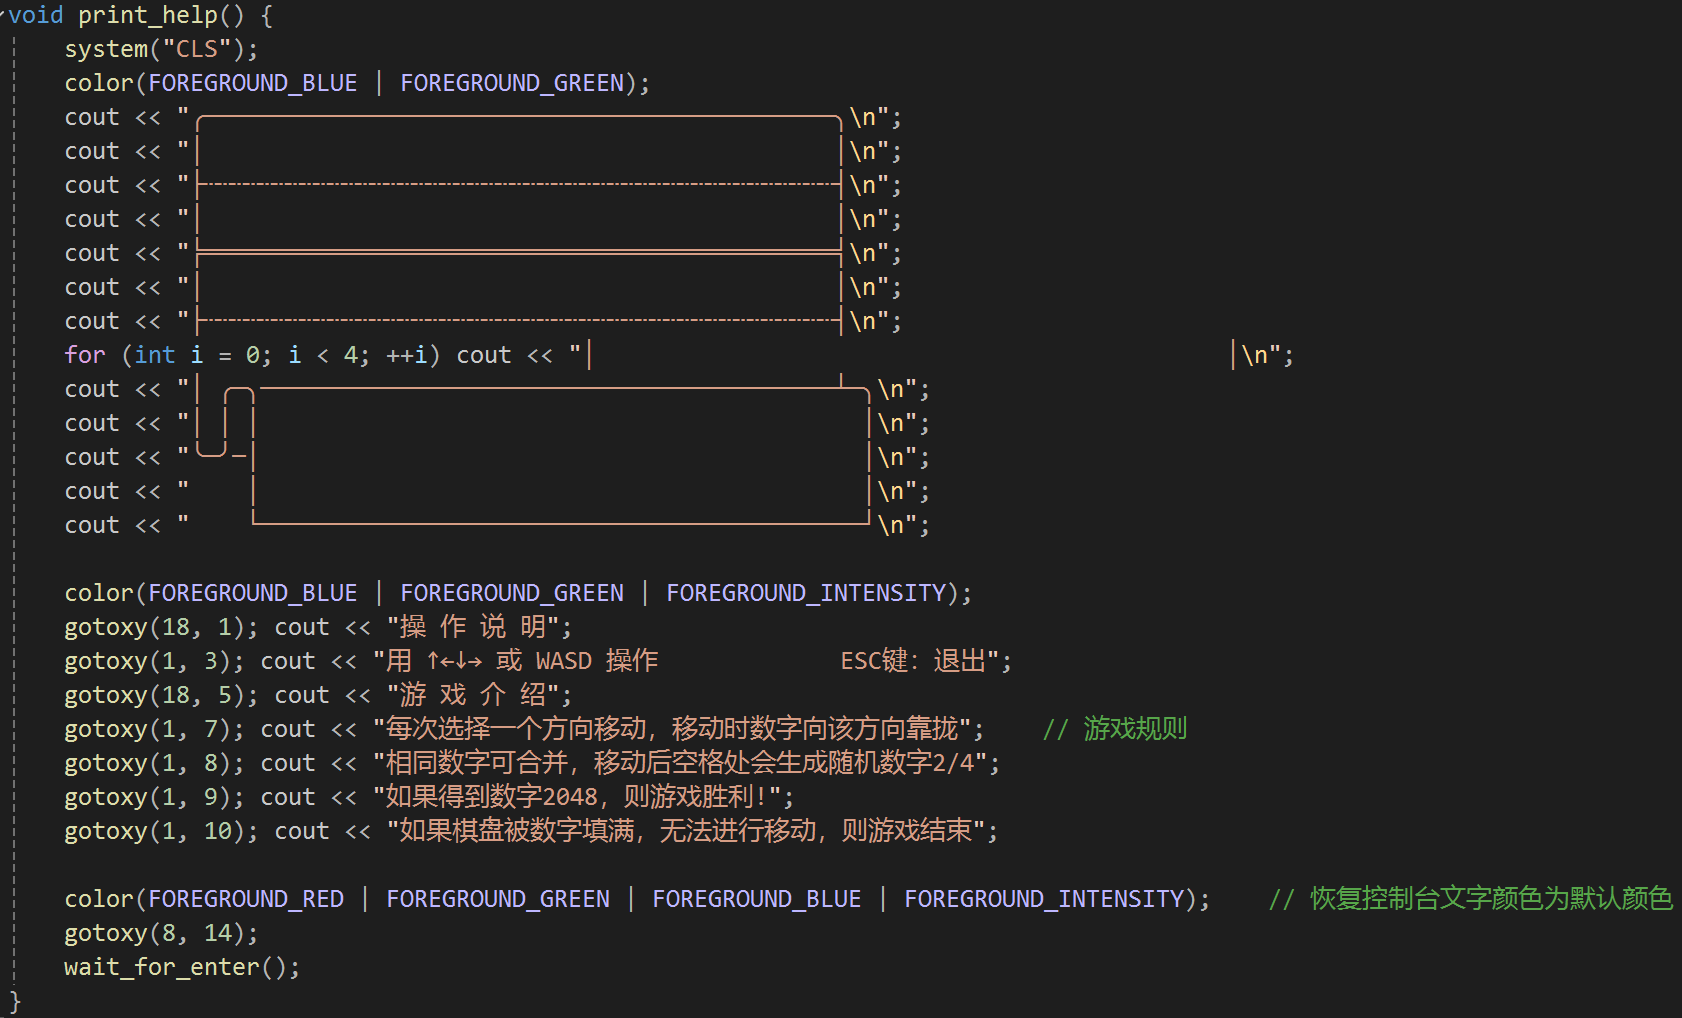
\includegraphics[width=.6\textwidth]{help.png}
    \caption{帮助}
\end{figure}

其次是程序的\textit{核心}部分,即游戏主循环:
\begin{lstlisting}[
    caption     =   {bf void play\_game()},
]
int board[4][4] = {}; // 4x4棋盘,并初始化
int score = 0;        // 分数
int step = 0;         // 步数
char choice = '\0';   // 用户选择
bool game_won = false; // 标志位,标记游戏是否已达2048

int high_score = read_high_score();    // 最高分

system("CLS");
print_interface();    // 打印游戏界面
update_board(board, score, step, high_score);
Sleep(200);
add_random_tile(board);     // 生成随机数并显示
add_random_tile(board);

while (1) {
    choice = _getch();        // 获取用户输入

    if (choice == 27) {  // 如果用户按下ESC键,跳出循环
        break;
    }

    // 根据用户输入进行相应操作
    if (move_tiles(board, choice, score)) {
        if (score > high_score) {      // 更新最高分
            high_score = score;
        }
        update_board(board, score, ++step, high_score);
        Sleep(200);
        add_random_tile(board);
    }

    // 检查是否达到了2048,如果还没有赢过游戏
    if (!game_won) {
        for (int i = 0; i < 4; i++) {
            for (int j = 0; j < 4; j++) {
                if (board[i][j] == 2048) {
                    game_won = true; // 设置游戏胜利标志
                    gotoxy(29, 18); cout << "\x1b[38;2;117;110;102;48;2;250;248;240m你赢了!";
                    gotoxy(27, 19); cout << "是否继续(y/n)";
                    while (1) {
                        choice = _getch();
                        if (choice == 'y' or choice == 'Y') {
                            gotoxy(29, 18); cout << "        ";
                            gotoxy(27, 19); cout << "             ";
                            break;
                        }
                        else if (choice == 'n' or choice == 'N') {
                            write_high_score(high_score); //写入最高分
                            return; //直接退出
                        }
                    }
                    break;
                }
            }
            if (game_won)
                break;
        }
    }

    // 检查是否还能移动方块,以判断游戏是否结束,若结束则跳出循环
    bool can_move = false;
    for (int i = 0; i < 4; ++i) {
        for (int j = 0; j < 4; ++j) {
            if (board[i][j] == 0)
                can_move = true;
            if (i < 3 && board[i][j] == board[i + 1][j])
                can_move = true;
            if (j < 3 && board[i][j] == board[i][j + 1])
                can_move = true;
        }
    }
    if (!can_move) {
        gotoxy(29, 18); cout << "\x1b[38;2;117;110;102;48;2;250;248;240m游戏结束!\n" << endl << endl;
        gotoxy(27, 19); wait_for_enter();
        break;
    }
}
write_high_score(high_score); //写入最高分
\end{lstlisting}

\subsection{游戏界面}
\begin{lstlisting}[
    caption     =   {背景颜色},
]
void background() {
    CONSOLE_SCREEN_BUFFER_INFO csbi;    // 获取控制台窗口尺寸
    int cols, rows;
    GetConsoleScreenBufferInfo(GetStdHandle(STD_OUTPUT_HANDLE), &csbi);
    cols = csbi.srWindow.Right - csbi.srWindow.Left + 1;
    rows = csbi.srWindow.Bottom - csbi.srWindow.Top + 1;

    cout << "\x1b[48;2;250;248;240m";
    for (int i = 0; i < rows; ++i) {
        for (int j = 0; j < cols; ++j) {
            cout << ' ';
        }
        cout << "\n";
    }
}
\end{lstlisting}

\begin{figure}[ht]
    \centering
    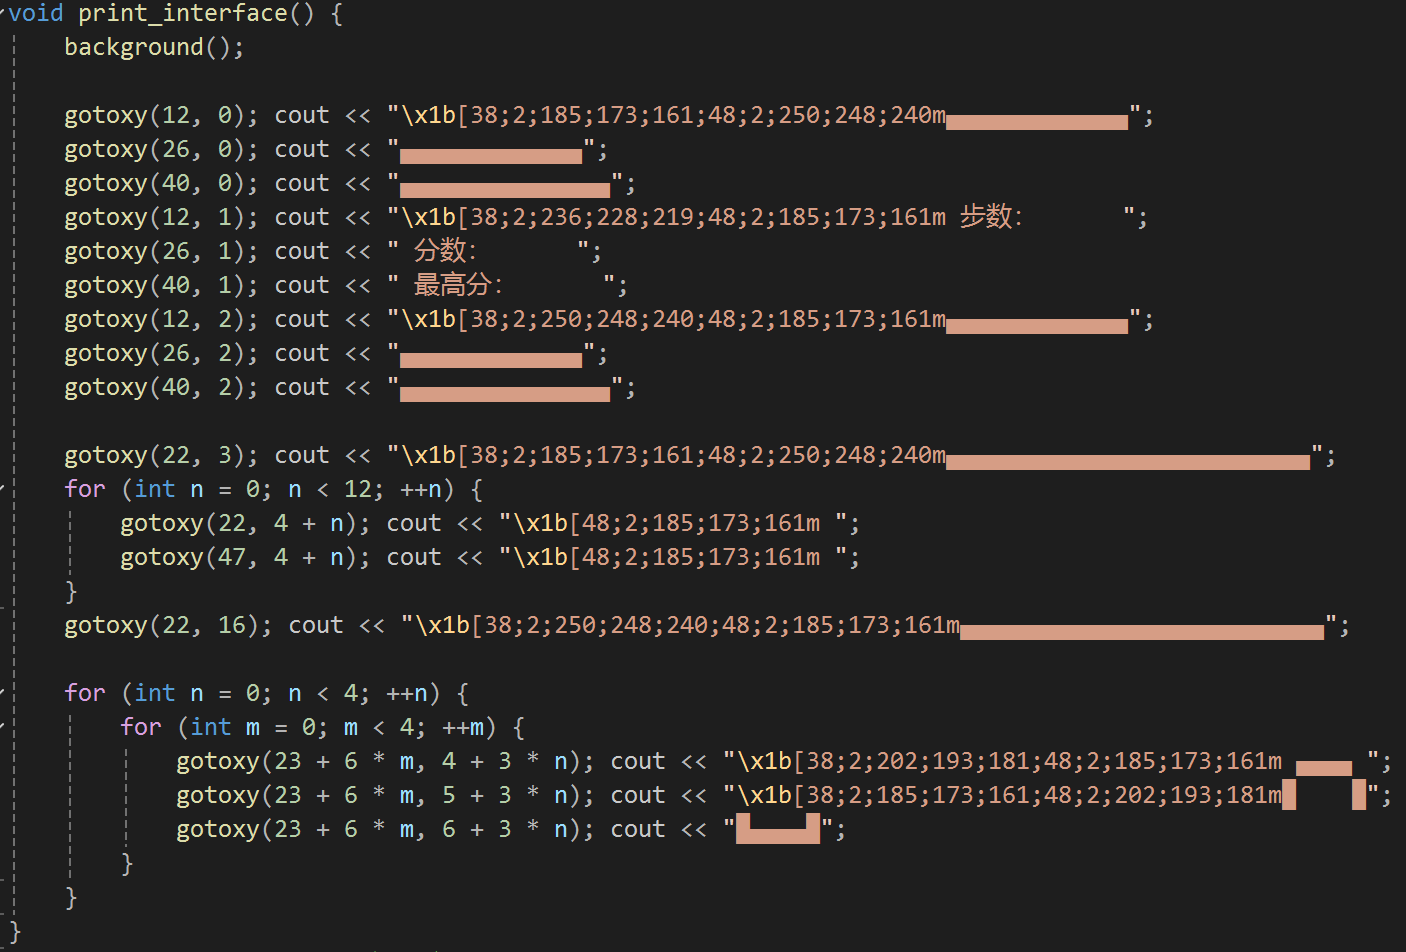
\includegraphics[width=.6\textwidth]{interface.png}
    \caption{游戏界面}
\end{figure}

\begin{lstlisting}[
    caption     =   {在棋盘上随机地添加随机数字 2/4 并显示},
]
void add_random_tile(int board[4][4]) {
    random_device rd; // 使用随机设备作为种子
    mt19937 gen(rd());    // 随机数生成器
    int empty_tiles[16][2];
    int count = 0;
    for (int i = 0; i < 4; ++i) {
        for (int j = 0; j < 4; ++j) {
            if (board[i][j] == 0) {
                empty_tiles[count][0] = i;
                empty_tiles[count][1] = j;
                count++;
            }
        }
    }

    if (count > 0) {
        int random_index = gen() % count;
        int x = empty_tiles[random_index][0];
        int y = empty_tiles[random_index][1];
        board[x][y] = (gen() % 10 + 10) % 10 > 0 ? 2 : 4; // 按概率比 9:1 随机生成 2 或 4
        display_tile(24 + y * 6, 5 + x * 3, board[x][y], 14);
    }
}
\end{lstlisting}

“根据用户操作,移动并倍增方块”的 \verb|move_tiles| 只部分展示:

\begin{lstlisting}[
    caption     =   {WASD 转换到方向键},
]
// 将 WASD 键映射到方向键,未与后方合并代码是考虑到保留动画
switch (direction) {
case 'w':
case 'W':
    direction = 72; break; // W -> 上
case 's':
case 'S':
    direction = 80; break; // S -> 下
case 'a':
case 'A':
    direction = 75; break; // A -> 左
case 'd':
case 'D':
    direction = 77; break; // D -> 右
}
\end{lstlisting}
随后再用一个 \verb|switch| 判断,比如,“上”的情况为
\begin{lstlisting}[
    caption     =   {上},
]
case 72: // 上
for (int j = 0; j < 4; ++j) {
    for (int i = 1; i < 4; ++i) {
        if (board[i][j] != 0) {
            int k = i;
            while (k > 0 && board[k - 1][j] == 0) {        // 移动
                move_with_animation(j, k, direction, board[k][j]);
                board[k - 1][j] = board[k][j];
                board[k][j] = 0;
                k--;
                moved = true;
            }
            if (k > 0 && board[k - 1][j] == board[k][j]) {        // 合并
                double_with_animation(j, k, direction, board[k][j]);
                board[k - 1][j] *= 2;
                score += board[k - 1][j];
                board[k][j] = 0;
                moved = true;
            }
        }
    }
}
break;
\end{lstlisting}


\begin{lstlisting}[
    caption     =   {更新数据},
]
void update_board(int board[4][4], int score, int step, int high_score) {
    gotoxy(18, 1);
    cout << "\x1b[38;2;255;255;255;48;2;185;173;161m" << setw(6) << step;
    gotoxy(32, 1);
    cout << setw(6) << score;
    gotoxy(48, 1);
    cout << setw(6) << high_score;

    for (int i = 0; i < 4; i++) {
        for (int j = 0; j < 4; j++) {
            display_tile(24 + j * 6, 5 + i * 3, board[i][j], 14);
        }
    }
}
\end{lstlisting}

移动 \verb|move_with_animation| 和倍增 \verb|double_with_animation| 也只部分展示:

\begin{figure}[ht]
    \centering
    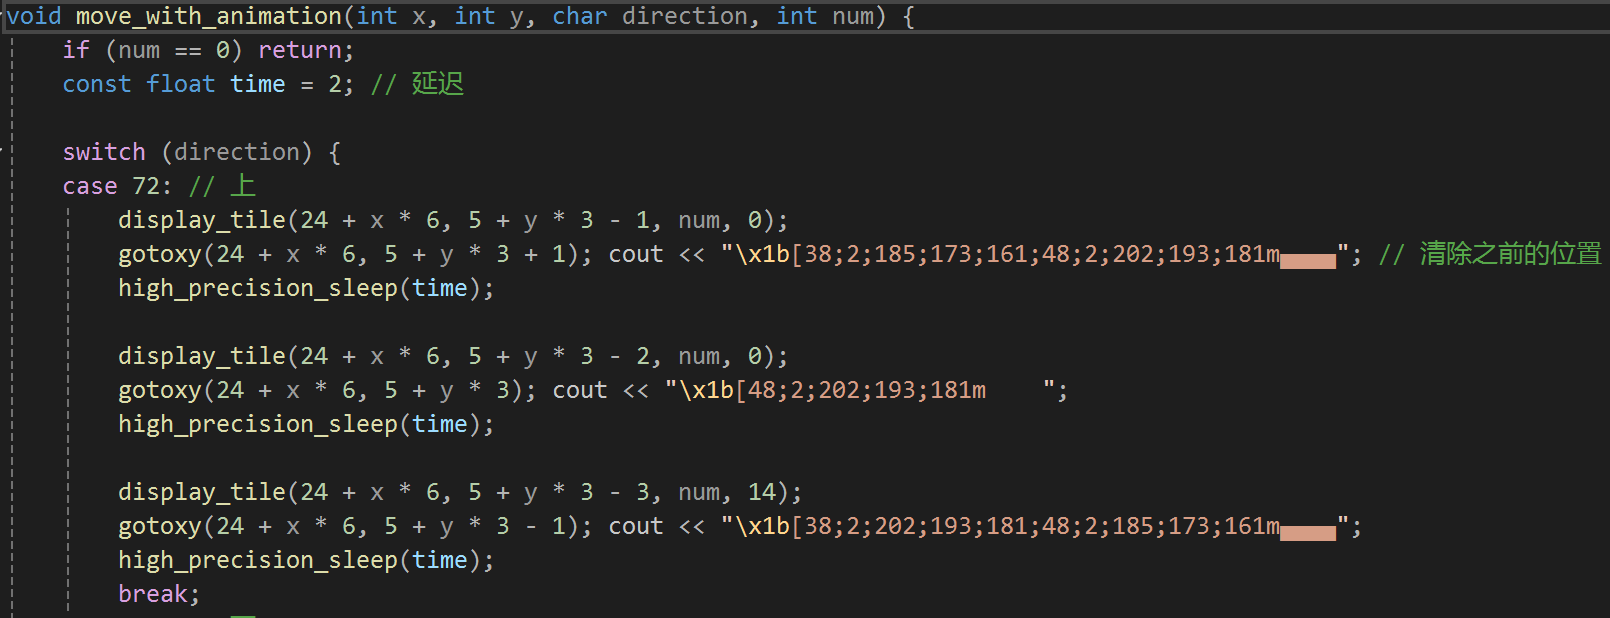
\includegraphics[width=.47\textwidth]{move_up.png}
    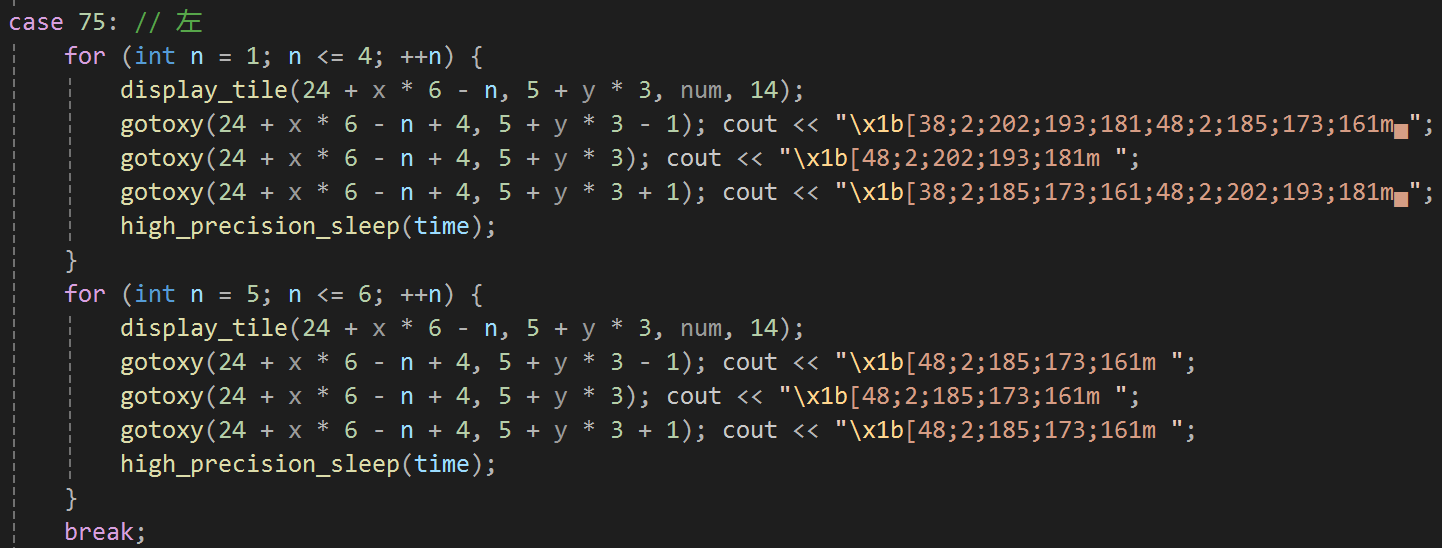
\includegraphics[width=.47\textwidth]{move_left.png}
    \caption{移动函数的“上”“左”}
\end{figure}


\begin{figure}[ht]
    \centering
    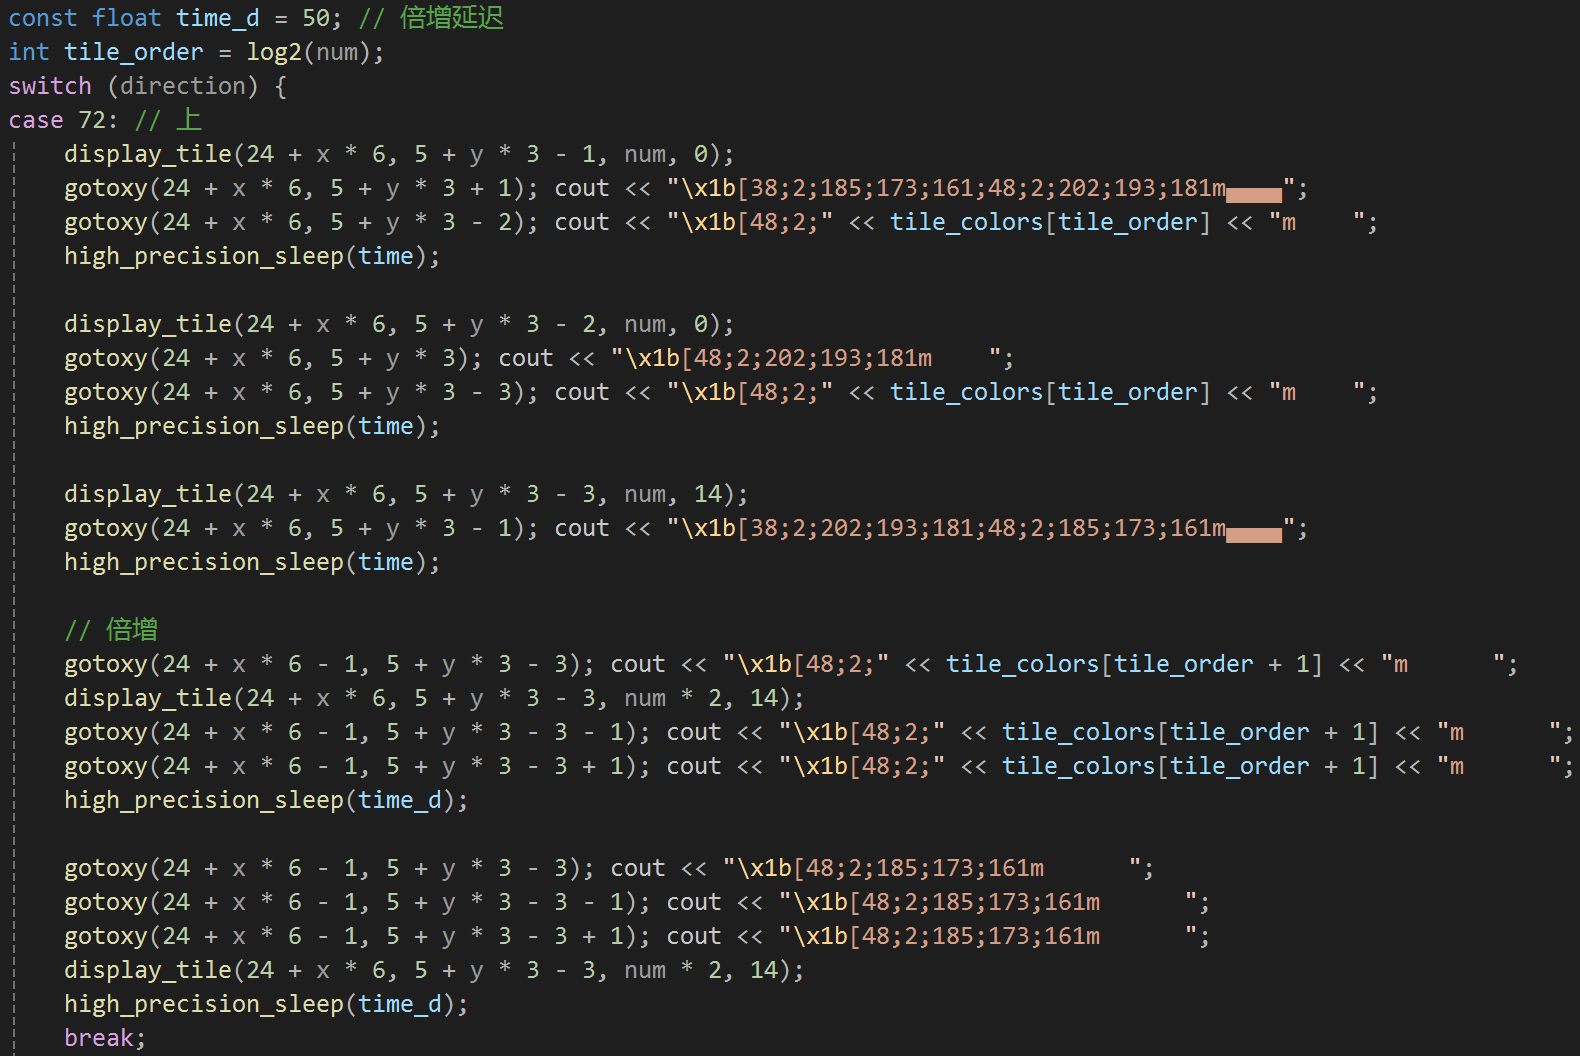
\includegraphics[width=.6\textwidth]{double_up.png}
    \caption{倍增函数的“上”}
\end{figure}

\begin{figure}[ht]
    \centering
    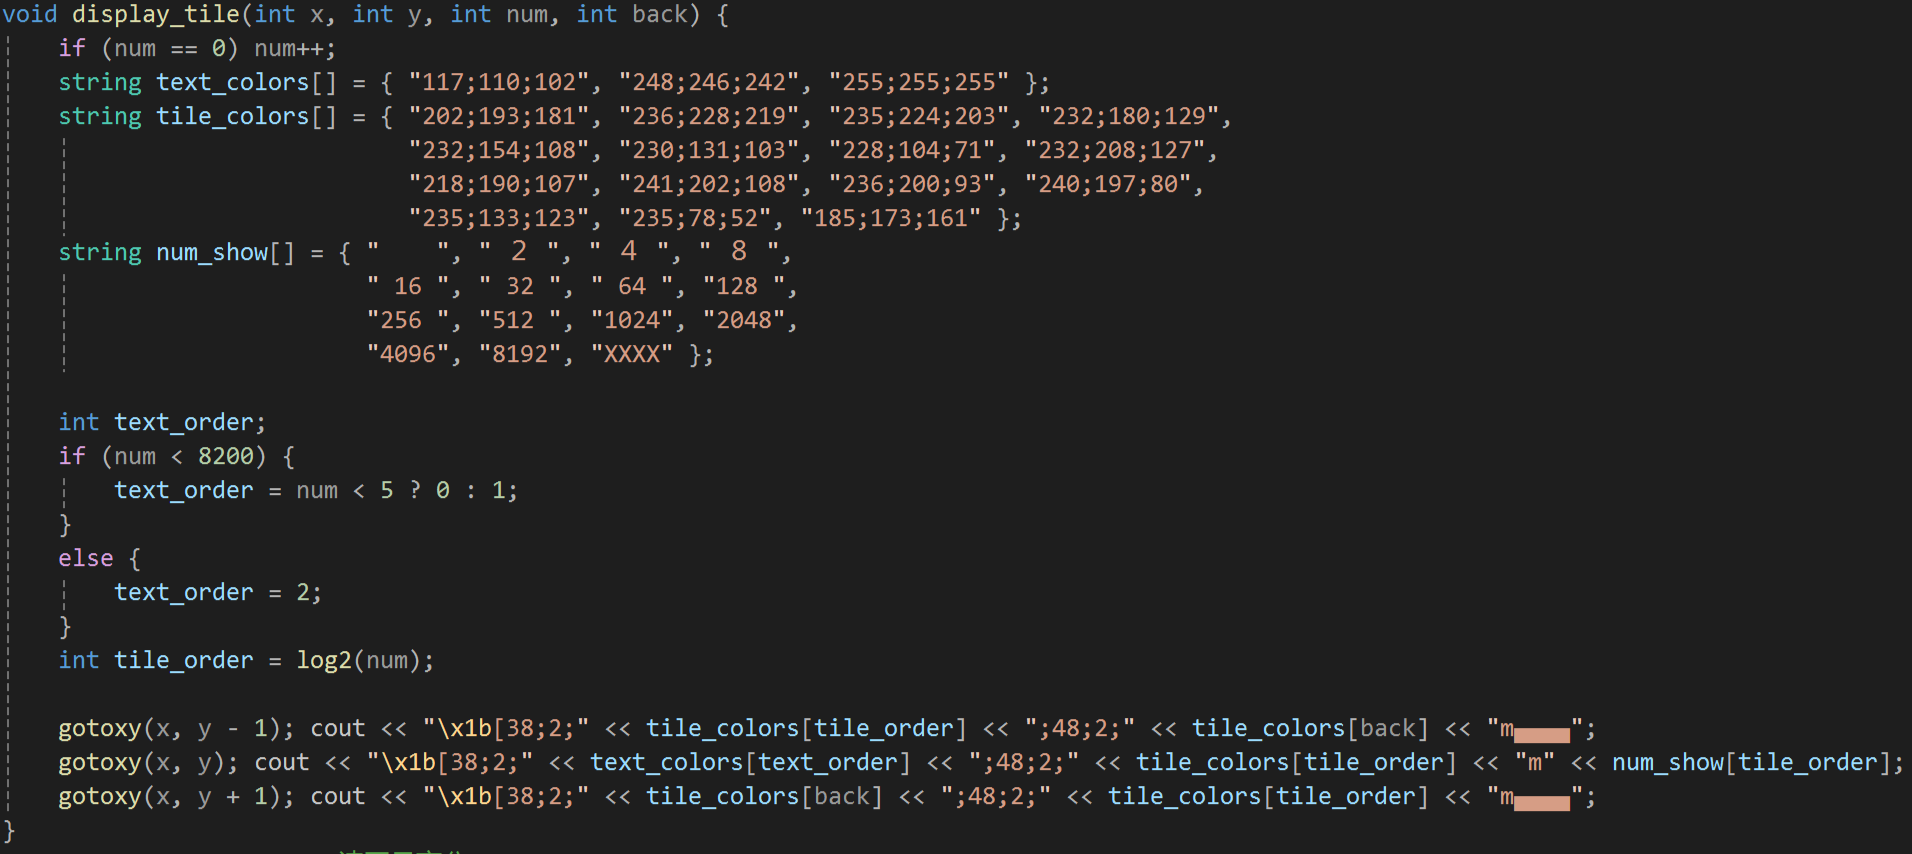
\includegraphics[width=.6\textwidth]{display.png}
    \caption{显示方块}
\end{figure}

\newpage
\subsection{其它函数}
这些函数是靠 AI 和搜索引擎获取的,十分方便:

\begin{lstlisting}[
    caption     =   {高精度延迟},
]
void high_precision_sleep(float milliseconds) {
    LARGE_INTEGER frequency;
    LARGE_INTEGER start, end;

    QueryPerformanceFrequency(&frequency);    // 获取高精度计时器的频率
    float wait_time = milliseconds * (frequency.QuadPart / 1000.0);    // 计算等待时间
    QueryPerformanceCounter(&start);    // 获取当前时间

    while (1) {
        QueryPerformanceCounter(&end);        // 获取当前时间
        float elapsed_time = (float)(end.QuadPart - start.QuadPart);        // 计算已过去的时间
        // 如果已过去的时间大于等于等待时间,退出循环
        if (elapsed_time >= wait_time)
            break;
    }
}
\end{lstlisting}

\begin{lstlisting}[
    caption     =   {读取最高分},
]
int read_high_score() {
    ifstream file("2048_highscore.txt");
    int high_score = 0;
    if (file.is_open()) {
        file >> high_score;
        file.close();
    }
    return high_score;
}
\end{lstlisting}

\begin{lstlisting}[
    caption     =   {写入最高分},
]
void write_high_score(int high_score) {
    ofstream file("2048_highscore.txt");
    if (file.is_open()) {
        file << high_score;
        file.close();
    }
}
\end{lstlisting}

\end{document}